\documentclass[aspectratio=169,10pt]{beamer}

\usetheme{lingnan}

\graphicspath{{../Long-Run Implications of Investment-Specific Technological Change/images/}}
\usepackage{tikz}
\usetikzlibrary{positioning}

\makeatletter
\renewcommand{\lingnansectionnav}{%
  \hbox to \paperwidth{%
    \lingnannavitem{1}{动机}{1}%
    \lingnannavitem{2}{模型}{2}%
    \lingnannavitem{3}{机制}{3}%
    \lingnannavitem{4}{结果}{4}%
    \lingnannavitem{5}{启示}{5}%
  }%
}
\makeatother

\title[\latinheading{Greenwood et al. (1997)}]{\latinheading{Long-Run Implications of\\Investment-Specific Technological Change}}
\subtitle{\latinheading{Greenwood, Hercowitz and Krusell (AER, 1997)}}
\author[Advanced Macro II pre]{赵天驰、郑文绰、邝逸、陈宇新、陈致远}
\institute{高级宏观经济学博士课程汇报}
\date[2026-06-16]{2026 年 6 月 16 日}

\newcommand{\paperfig}[3]{%
  \begin{figure}
    \centering
    \includegraphics[width=#1\linewidth,height=0.56\textheight,keepaspectratio]{#2}
    \caption{\scriptsize #3}
  \end{figure}
}

\begin{document}

\begin{frame}[plain]
  \titlepage
\end{frame}

\section{\latinheading{动机和背景}}

\begin{frame}{现实背景}
  \begin{columns}[T,onlytextwidth]
    \begin{column}{0.27\linewidth}
      \centering
      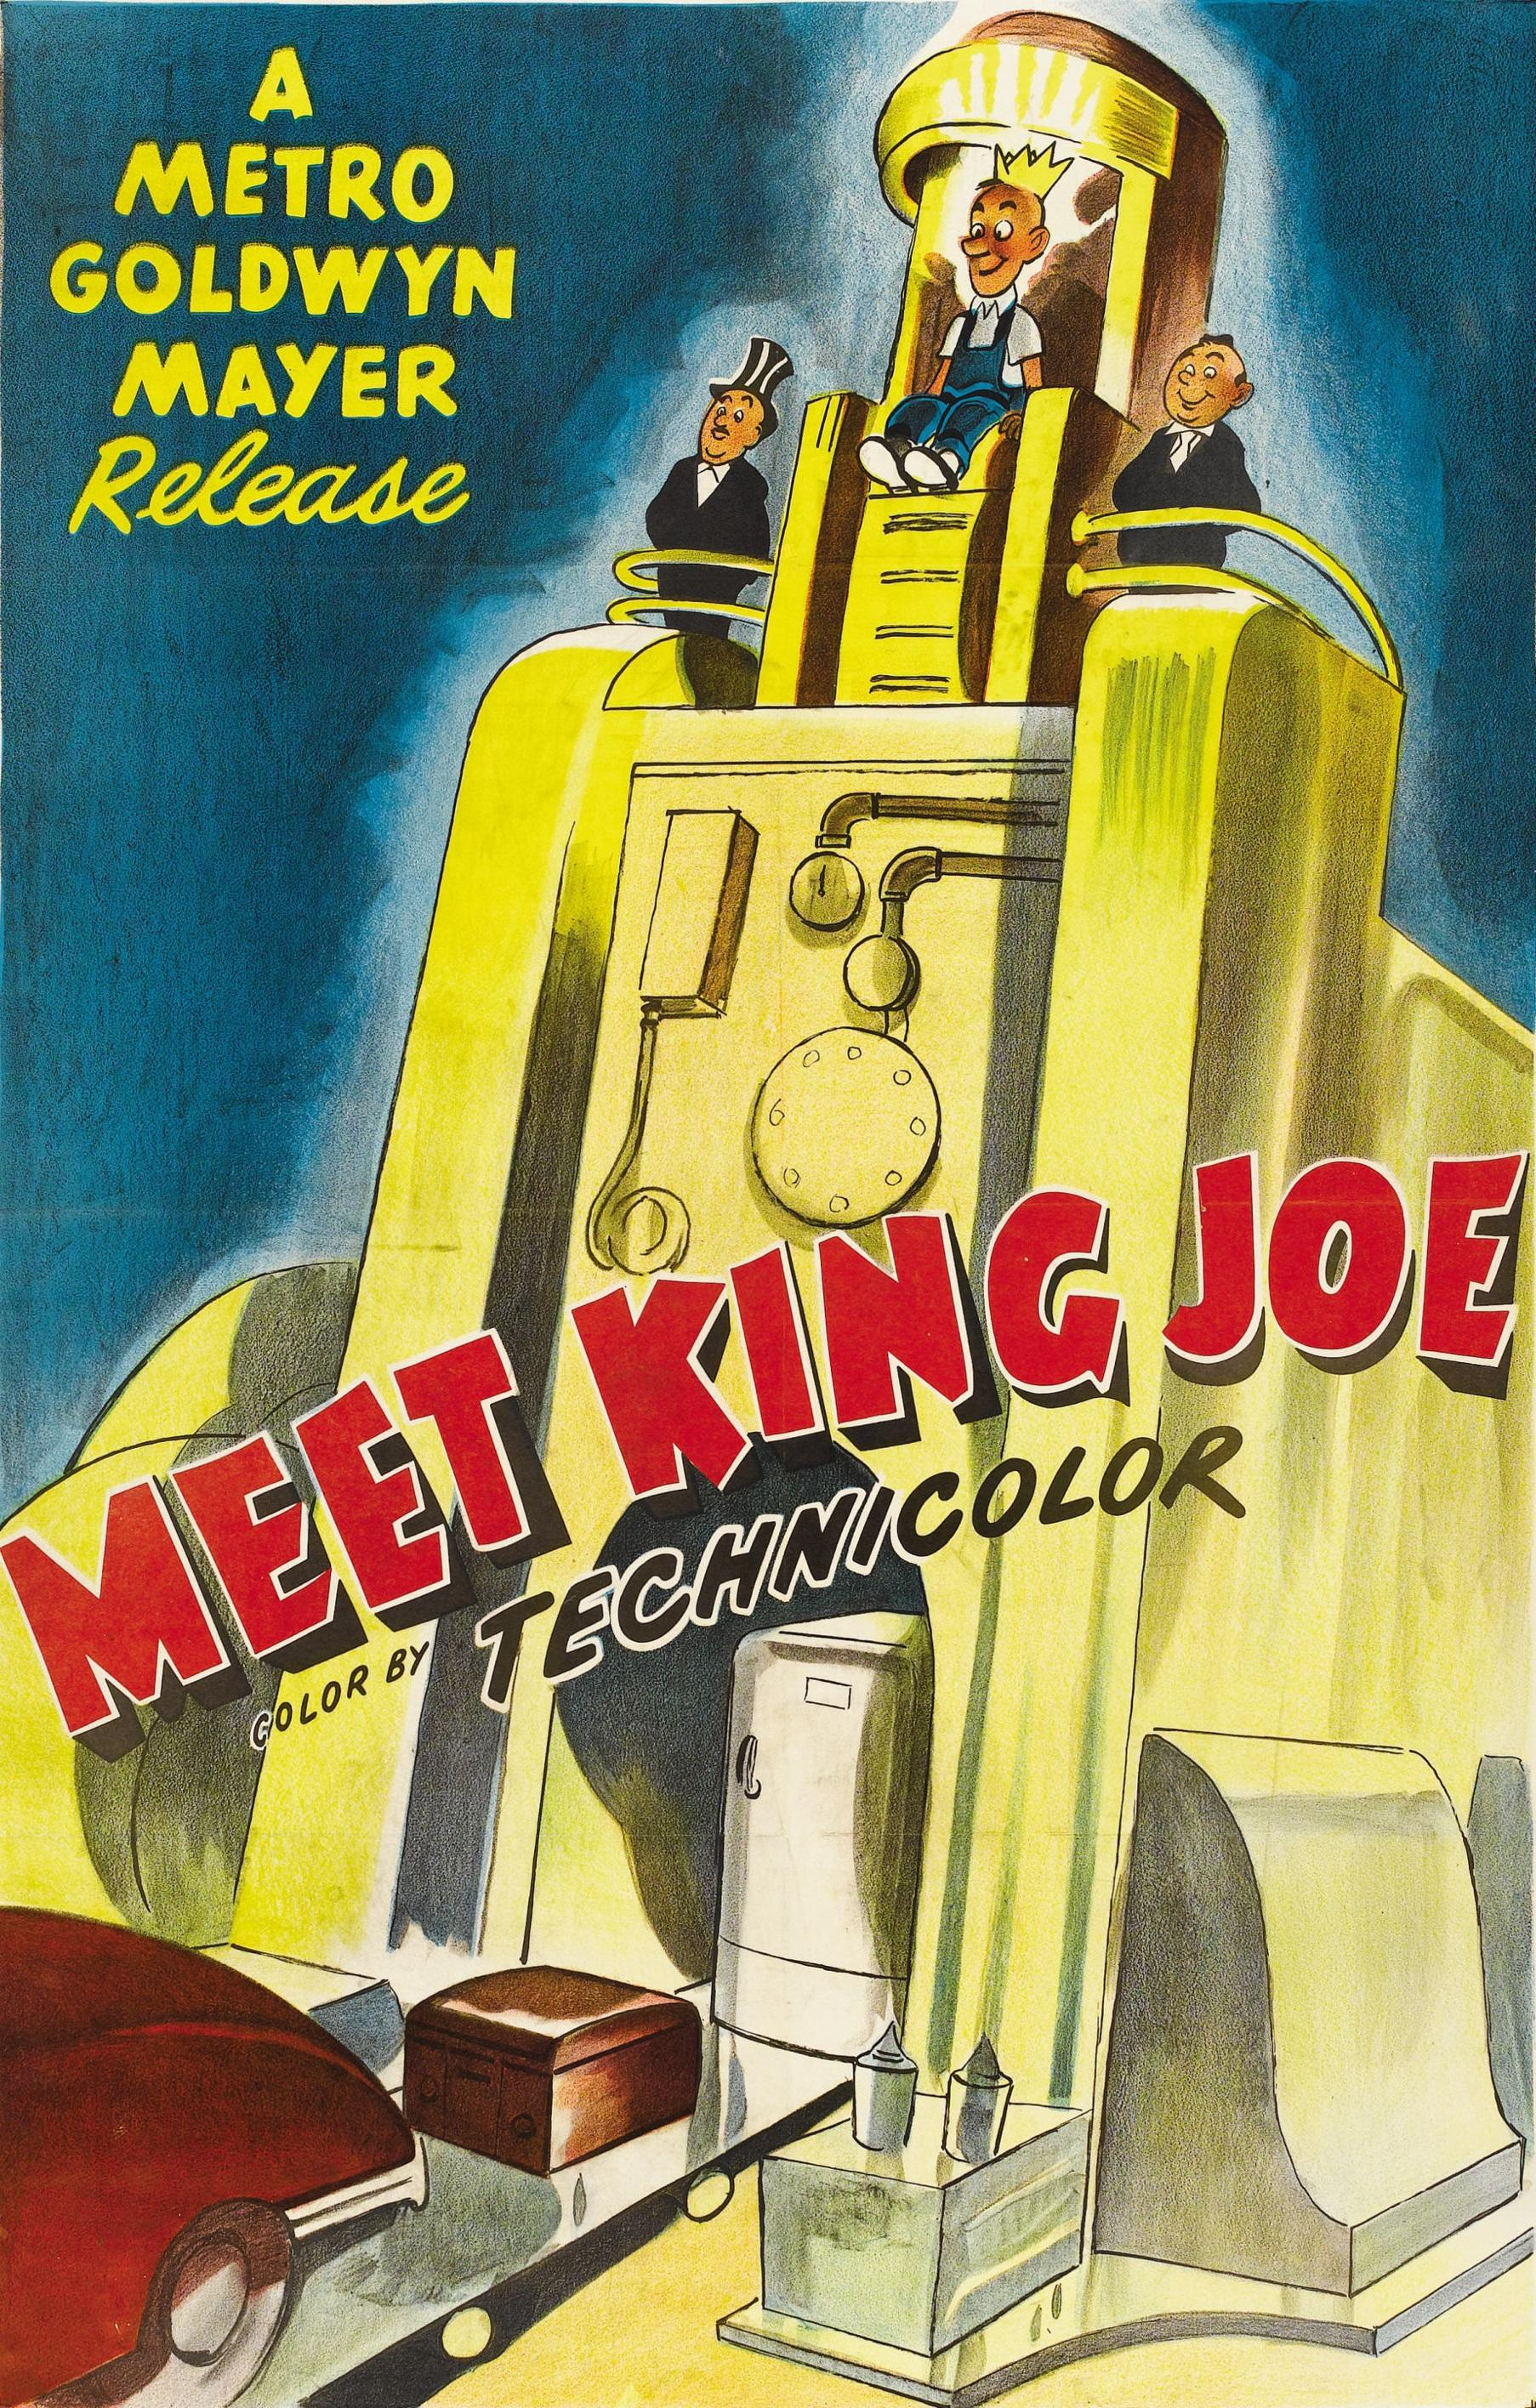
\includegraphics[width=\linewidth,height=0.58\textheight,keepaspectratio]{image/1949.jpg} \\
      {\scriptsize 1949年}
    \end{column}

    \begin{column}{0.42\linewidth}
      % \scriptsize
      \vspace{1em}
      \begin{enumerate}
        \item 二战后的黄金增长（1945--1973）
              \begin{itemize}
                \item TFP 年均增速达 2\%
                \item TFP 贡献超过 50\%
              \end{itemize}
        \item 此后，增速全面下滑（1973-1995）
              \begin{itemize}
                \item 1965-1973 为 1.5\%
                \item 1973-1995 为 0.6\%
              \end{itemize}
        \item 同时，技术蓬勃发展
              \begin{itemize}
                \item 1968 年 Intel 成立；
                \item 1985 年高通成立。
              \end{itemize}
      \end{enumerate}
      \vspace{-0.4em}
    \end{column}

    \begin{column}{0.27\linewidth}
      \centering
      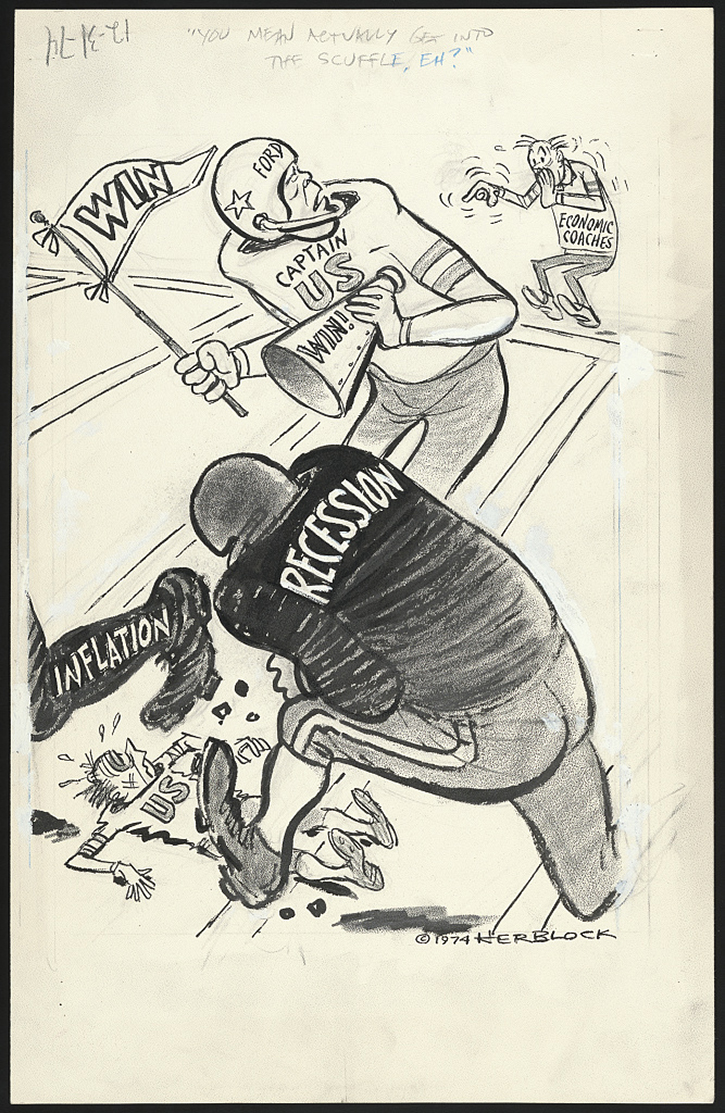
\includegraphics[width=\linewidth,height=0.58\textheight,keepaspectratio]{image/1974.jpg} \\
      {\scriptsize 1974年}
    \end{column}
  \end{columns}
  \begin{block}{}
    \begin{center}
      \textbf{索洛悖论：}You can see the computer everywhere but in the productivity statistics.
    \end{center}
  \end{block}
\end{frame}

\begin{frame}{两个重要的问题}

  \vspace{0.45cm}

  \begin{columns}[c,onlytextwidth]
    \begin{column}{0.48\linewidth}
      \begin{block}{问题一：长期增长解释}
        \centering
        \vspace{0.18cm}

        {\Large 如何理解经济增长？}

        \vspace{0.25cm}

        % {%\small
        %   技术进步与资本积累并非孤立
        % }

        \vspace{0.18cm}
      \end{block}
    \end{column}

    \begin{column}{0.48\linewidth}
      \begin{block}{问题二：生产率谜题}
        \centering
        \vspace{0.18cm}

        {\Large 如何解释索罗悖论？}

        \vspace{0.25cm}

        % {%\small
        %   生产率测量不够精细
        % }

        \vspace{0.18cm}
      \end{block}
    \end{column}
  \end{columns}

  % \vfill

  \begin{block}{}
    \begin{center}
      \Large \textbf{一个洞见}
    \end{center}
  \end{block}

\end{frame}

\begin{frame}{典型事实：投资价格和占比的负向关系}
  \begin{columns}[T,onlytextwidth]
    \begin{column}{0.48\linewidth}
      \begin{itemize}
        \item 设备价格越来越低，投资数量却越来越高
      \end{itemize}
      \paperfig{0.98}{fig1_investment_in_equipment.jpg}{Investment in Equipment}
    \end{column}
    \begin{column}{0.48\linewidth}
      \begin{itemize}
        \item 去除趋势后，负向的相关关系依然成立
      \end{itemize}
      \paperfig{0.98}{fig2_investment_hp_detrended.jpg}{Investment in Equipment, HP Detrended}
    \end{column}
  \end{columns}
\end{frame}

\begin{frame}{传统模型：难以解释现有事实}

  \begin{block}{现有事实}
    \begin{itemize}
      \item 设备（投资）相对价格上升（$r/p^c \uparrow$）
      \item 设备（投资）占比下降（$I^i/Y \downarrow$）
      \item 二者存在负向的相关性，是谁影响了谁？是否可能来自于同一个因素的影响？
    \end{itemize}
  \end{block}
  \begin{block}{传统模型局限：假设处于平衡增长路径上恒定}
    \begin{itemize}
      \item 投资占产出比重不变（平衡增长路径）
            $$ \eta \equiv \frac{I_t}{Y_t} =(g-1+\delta)\frac{K_{t}}{Y_t} $$
      \item 投资相对消费价格不变（资本边际收益 = 边际产出）
            $$ r_t = p^{c}_t \times \alpha_{K} \dfrac{Y_t}{K_{t}} $$

    \end{itemize}
  \end{block}
\end{frame}

\begin{frame}{如何解释？}
  \begin{itemize}
    \item 我们的一些尝试：首先明确，\textbf{供给侧层面}的\textbf{价格冲击}
  \end{itemize}
  \begin{columns}[T,onlytextwidth]
    \begin{column}{0.31\linewidth}
      \centering
      
\includegraphics[width=\linewidth,height=0.58\textheight,keepaspectratio]{\detokenize{image/军器民用.png}}
      \vspace{0.1em}
      \textbf{军器民用：产业技术进步}
    \end{column}

    \begin{column}{0.31\linewidth}
      \centering
      
\includegraphics[width=\linewidth,height=0.58\textheight,keepaspectratio]{\detokenize{image/管制放松.png}}
      \vspace{0.1em}
      \textbf{管制放松：国内竞争加剧}
    \end{column}

    \begin{column}{0.31\linewidth}
      \centering
      
\includegraphics[width=\linewidth,height=0.58\textheight,keepaspectratio]{\detokenize{image/贸易自由.png}}
      \vspace{0.1em}
      \textbf{贸易自由：国外厂商进入}
    \end{column}
  \end{columns}
\end{frame}

\begin{frame}[t]{文中的解释：投资特定的技术进步}

  \begin{columns}[T,onlytextwidth]
    \begin{column}{0.48\linewidth}
      \vspace{2em}
      \begin{block}{}
        \begin{center}
          \large 投资特定的技术进步（Investment-Specific Technological Change）
        \end{center}
      \end{block}
      \vspace{0.5em}
      \begin{enumerate}
        \item 特定的
              \begin{itemize}
                \item 存在\textbf{非中性的}技术进步
              \end{itemize}
        \item 投资特定的
              \begin{itemize}
                \item 体现在\textbf{新设备的质量提升}和价格下降
                \item 消费和服务受到的影响较小
                \item 厂房和基础设施等资本无明显变化
              \end{itemize}
      \end{enumerate}

    \end{column}

    \begin{column}{0.48\linewidth}
      \centering
      
\includegraphics[width=0.9\linewidth,keepaspectratio]{\detokenize{image/技术进步示意.png}}
    \end{column}
  \end{columns}
\end{frame}

\section{\latinheading{模型设定}}

\begin{frame}{消费端}
  \begin{block}{效用函数}
    \begin{itemize}
      \item 家庭最大化预期效用
            \begin{equation}
              \max \; \left[E\sum_{t=0}^{\infty}\beta^t U(c_t,l_t)\right].
            \end{equation}
      \item 效用由消费和劳动决定
            \begin{equation}
              U(c,l)=\theta \ln c+(1-\theta)\ln(1-l).
            \end{equation}
            \begin{itemize}
              \item $c_t$：消费。
              \item $l_t$：劳动投入，$1-l_t$ 是闲暇。
            \end{itemize}
    \end{itemize}
  \end{block}
\end{frame}

\begin{frame}{生产端}


  \begin{block}{生产函数}
    \begin{equation}
      \begin{gathered}
        y = z \cdot \textcolor{ModernRed}{k_e^{\alpha_e}k_s^{\alpha_s}} \cdot l^{1-\alpha_e-\alpha_s}, \\
        0 < \alpha_e+\alpha_s < 1.
      \end{gathered}
    \end{equation}

    \begin{itemize}
      \item $k_e$：设备资本 (equipment)，更新快、改进明显；如机器设备、计算机、生产线、运输设备。
      \item $k_s$：结构资本 (structures)，更耐久、进步较慢；如厂房、办公楼、道路等建筑和基础设施。
    \end{itemize}
  \end{block}

  % \begin{block}{市场出清}
  %   \begin{equation}
  %     y=c+i_e+i_s.
  %   \end{equation}
  % \end{block}

  \keymessage{主要创新}{$k \to k_e, k_s$, 将设备资本和结构资本区分开来，允许它们承载不同的技术进步。}

\end{frame}

\begin{frame}{生产端}

  \begin{block}{资本积累}
    \begin{itemize}
      \item 结构资本：基本上没有明显的技术进步，单位投资形成 $1$ 单位结构资本。
            \begin{equation}
              k_s'=(1-\delta_s)k_s+i_s
            \end{equation}
      \item \textbf{设备资本}：技术进步快，单位投资形成$q$ 单位设备资本。
            \begin{equation}
              k_e'=(1-\delta_e)k_e+ \textcolor{ModernRed}{q} \cdot i_e
            \end{equation}
            \begin{itemize}
              \item $q$ 新一代产品的技术或效率（价格不变）
              \item ${1}/{q}$ 新一代产品的价格（质量不变）
            \end{itemize}
      \item $\delta_s, \delta_e \in (0,1)$ 折旧率。
    \end{itemize}
  \end{block}


\end{frame}

\begin{frame}{政府}

  \begin{block}{税收方程}

    \begin{equation}
      \tau=\tau_k(r_e k_e+r_s k_s)+\tau_l w l.
    \end{equation}
    \begin{itemize}
      \item 政府对劳动和资本收入征税，税率分别为 $\tau_l$ 和 $\tau_k$。
      \item $r_e$ 和 $r_s$ ：$k_e$和$k_s$的回报率。
      \item $w$：劳动的工资率。
      \item 政府不进行消费和借贷，只进行转移支付。
    \end{itemize}
  \end{block}

  \keymessage{设置税收的目的}{校准现实经济：税收影响家庭的决策，进而影响资本积累和增长路径。}

\end{frame}

\begin{frame}{模型设定：为什么要和为什么能？}
  \begin{block}{为什么要？}
    对资本类型进行区分（加入 $q$）后，设备资本的效率增加时有：
    \begin{itemize}
      \item 设备的相对价格下降：
            $$ r_{e,t} \downarrow = \dfrac{p^c_t}{q \uparrow} \times \alpha_{K_e} \dfrac{Y_t}{K_{e,t}} $$
      \item 设备的相对占比提高：
            $$ \frac{i_e}{y} \uparrow = (g-1+\delta_e)\frac{k_e}{y} \times q \uparrow$$
    \end{itemize}
  \end{block}

  \begin{block}{为什么能？}
    \begin{itemize}
      \item 现实支持：资本的使用效率存在区别（厂房 vs 设备）。
      \item 数据支持：Gordon's equipment price index 提供了设备价格。
      \item 理论支持：拆分后，可以使用符合生产函数，依然能有对应模型。
    \end{itemize}
  \end{block}

\end{frame}

\section{模型求解与参数估计}
% \subsection{竞争均衡与平衡增路径}

\begin{frame}{模型总结}
  \small
  \begin{block}{消费者跨期效用最大化}
    \begin{equation*}
      \begin{aligned}
        V(k_e, k_s; s, z, q)                   & = \max_{c, k'_e, k'_s, l} \left\{  U(c,l) + \beta E[V(k'_e, k'_s; s', z, q)] \right\}     \\
        s.t. \quad  c + \dfrac{k'_e}{q} + k'_s & = (1- \tau_k)\left[R_e(\lambda) k_e  + R_s (\lambda) k_s \right] + (1-\tau_l)W(\lambda) l \\
                                               & + (1-\delta_e)\dfrac{k_e}{q} + (1-\delta_s)k_s + T(\lambda)                               \\
        k'_s                                   & = (1-\delta_s)k_s + i_s                                                                   \\
        k'_e                                   & = (1-\delta_e)k_e + q i_e
      \end{aligned}
    \end{equation*}
  \end{block}

  \begin{block}{厂商利润最大化}
    \begin{equation*}
      \max_{\tilde{k}_e, \tilde{k}_s, \tilde{l}} \pi_y = z F(\tilde{k}_e, \tilde{k}_s, \tilde{l}) - R_e(\lambda) \tilde{k}_e - R_s(\lambda) \tilde{k}_s - W(\lambda)\tilde{l}
    \end{equation*}
  \end{block}


\end{frame}



\begin{frame}{竞争性均衡}
  \small
  \begin{block}{状态变量}
    $$\lambda = (s, z, q), \qquad s\equiv(k_e, k_s)$$
    \vspace{-1.2em}
    \begin{itemize}
      % \item 当前状态主要由三个变量决定：$s$（资本存量），$z$:（TFP），$q$（设备效率）。
      \item 当期状态将决定下一期状态：
            \begin{itemize}
              \item $s' \equiv S(\lambda) = (k'_e, k'_s) = (K_e(\lambda), K_s(\lambda)) $ 由资本积累方程决定。
              \item $z'$ 和 $q'$ 由外生过程决定，增长率为 $\gamma_z$ 和 $\gamma_q$。
            \end{itemize}
    \end{itemize}
  \end{block}

  \begin{block}{模型求解}
    \begin{itemize}
      \item 消费者最优：$c = C(\lambda)$, $k'_e = K_e(\lambda)$，$k'_s = K_s(\lambda)$, $l = L(\lambda)$
      \item 生产者最优：$\tilde{k}_e =  \tilde{K}_e(\lambda)$, $\tilde{k}_s = \tilde{K}_s(\lambda)$, $\tilde{l} = \tilde{L}(\lambda)$
      \item 市场出清：$k_e = \tilde{k}_e$, $k_s = \tilde{k}_s$, $l = \tilde{l}$, $zF(k_e, k_s, l) = c + i_e + i_s$
            \begin{itemize}
              \item 要素价格：$w = W(\lambda)$，$r_e = R_e(\lambda)$，$r_s = R_s(\lambda)$ $ \Rightarrow \qquad \tau = T(\lambda)$
            \end{itemize}
    \end{itemize}
  \end{block}

\end{frame}

\begin{frame}{平衡增长的定义}
  \small
  \begin{block}{外生的技术进步：$\gamma_z$ 和 $\gamma_q$}

    \begin{equation*}
      z_t \equiv \gamma_z^t \qquad q_t \equiv \gamma_q^t
    \end{equation*}
  \end{block}
  \begin{block}{平衡增长速度：$g$}
    \begin{equation*}
      g \equiv \dfrac{y_{t+1}}{y_t}  = \dfrac{c_{t+1}}{c_{t}} = \dfrac{i_{s,t+1}}{i_{s,t}} = \dfrac{i_{e,t+1}}{i_{e,t}}
    \end{equation*}
    为什么 $y$, $c$, $i_s$, $i_e$ 增速一定相同，但是对 $k_s$, $k_e$ 的增速则无要求？
    \begin{itemize}
      \item 资源限制方程：$y = c + i_s + i_e$（与 $k_s$ 和 $k_e$ 无关），以 $c$ 为例进行说明
      \item 若 $g_y > g_c$，消费占比会趋于0，出现资源的冗余；
      \item 若 $g_y < g_c$，消费占比会趋于无穷，超出资源约束。
    \end{itemize}
  \end{block}
\end{frame}

\begin{frame}{平衡增长的联系}
  \small
  \begin{block}{资本增速$g_s = g$，$g_e = g\gamma_q$}
    \begin{equation*}
      k_s = (1-\delta_s)k_s + i_s \Rightarrow g_s = (1-\delta_s) + \dfrac{i_s}{k_s} \Rightarrow k_s = g
    \end{equation*}
    因为若 $g_s$ 为常数，则 $i_s/k_s$ 必为常数，$k_s$ 与 $i_s$ 同速率增长。
    \begin{equation*}
      g_e = (1-\delta_s) + \dfrac{q i_s}{k_s} \Rightarrow g_e = g \gamma_q
    \end{equation*}
  \end{block}

  \begin{block}{增长速率的表示}
    将生产函数写成增速的表达形式：
    \begin{equation*}
      g = \gamma_z^{1/(1-\alpha_e - \alpha_s)} \gamma_q^{\alpha_e/(1-\alpha_e - \alpha_s)}
    \end{equation*}
    \begin{equation*}
      g_e = \gamma_z^{1/(1-\alpha_e - \alpha_s)} \gamma_q^{(1-\alpha_s)/(1-\alpha_e - \alpha_s)}
    \end{equation*}
  \end{block}

\end{frame}


% \subsection{参数估计}

\begin{frame}{待估参数}
  % \scriptfont
  % \small
  \begin{columns}[T,onlytextwidth]
    \begin{column}{0.37\linewidth}
      \begin{block}{待估参数汇总（4/16）}
        \begin{enumerate}
          \item 家庭端：${\beta}, {\theta}$
          \item 生产端：$\mathhighlight{\delta_e, \delta_s}, {\alpha_e}, {\alpha_s}$
          \item 政府端：$\mathhighlight{\tau_l}, \tau_k$
          \item 增长率：$\mathhighlight{\gamma_q}, \gamma_z, g$
          \item 要素份额：$\dfrac{\hat{c}}{\hat y}, \dfrac{\hat{i}_e}{\hat y}, \dfrac{\hat{i}_s}{\hat y},  \dfrac{\hat{k}_e}{\hat y}, \dfrac{\hat{k}_s}{\hat y}$
        \end{enumerate}
      \end{block}
      % \begin{block}{内生变量汇总}
      %   \begin{enumerate}
      %     \item 家庭端：$c_t, l_t$
      %     \item 生产端：$y_t, k_{e,t}, k_{s,t}$
      %   \end{enumerate}
      % \end{block}
    \end{column}
    \begin{column}{0.57\linewidth}
      \vspace{1em}
      \begin{enumerate}
        \item[1.] 技术进步（$\gamma$）：$\gamma_q = 1.032$
              \begin{equation*}
                \gamma_q = \dfrac{q_{t+1}}{q_t} =  \dfrac{\mathhighlight{r_{e,t}}}{\mathhighlight{r_{e,t+1}}}
              \end{equation*}
              $r_{e}$ 数据来源于 Gordon's equipment price index。
        \item[2-3.] 折旧率（$\delta$）：$\delta_s = 0.056$，$\delta_e = 0.124$
              \begin{equation*}
                \mathhighlight{k_{t}} = (1-\delta) \mathhighlight{k_{t-1}}
              \end{equation*}
              $k_t$ 数据来源于 BEA。
        \item[4.] 税率（$\tau$）：$\tau_l = 0.40$ \\
              参考现有研究（Robert E. Lucas, 1990）。
      \end{enumerate}

    \end{column}
  \end{columns}

\end{frame}

\begin{frame}{参数估计}
  \begin{block}{}
    \begin{center}
      待估参数（7/16）：$\boxed{\mathhighlight{
            \delta_e, \delta_s,  \tau_l, \gamma_q} \qquad \mathhighlight{\gamma_z, g, (\alpha_e+\alpha_s)} \qquad  \theta, \beta, \tau_k, \dfrac{\hat{i}_e}{\hat{y}}, \dfrac{\hat{i}_s}{\hat{y}}, \dfrac{\hat{k}_e}{\hat{y}}, \dfrac{\hat{k}_s}{\hat{y}}, \dfrac{\hat{c}}{\hat{y}} }$
    \end{center}
  \end{block}
  \begin{itemize}
    \item[5.] 平衡增长（$g = 1.24$）：年度 GNP 增长率数据。
          \begin{equation*}
            g = 1.24
          \end{equation*}
          % \item 劳动参与：$l = 0.24$，使用每周工作小时数占非睡眠时间的比例。
    \item[6.] 资本份额（$\alpha_e+ \alpha_s = 0.30$）：资本收入份额数据。
          \begin{equation*}
            \alpha_e + \alpha_s = 0.30
          \end{equation*}
    \item[7.] 技术进步（$\gamma_z$）
          \begin{equation*}
            g = \gamma_z g^{\alpha_e+\alpha_s} \gamma_q^{\alpha_e} \Rightarrow
            \gamma_z = \dfrac{\mathhighlight{g}^{1-\mathhighlight{(\alpha_e + \alpha_s)}}}{\mathhighlight{\gamma_{q}^{\alpha_e}}} \qquad \boxed{k_e \text{平衡增长路径}}
          \end{equation*}


          % \item 设备投资占比：$i_e/y = 0.073$，使用设备投资占 GNP 的比例。
          % \item 结构投资占比：$i_s/y = 0.041$，使用结构投资占 GNP 的比例。
  \end{itemize}

\end{frame}

\begin{frame}{参数估计}
  \begin{block}{}
    \begin{center}
      待估参数（9/16）：$\boxed{\mathhighlight{
            \delta_e, \delta_s,  \tau_l, \gamma_q,  (\alpha_e+\alpha_s), \gamma_z, g} \qquad \mathhighlight{\beta, \theta} \qquad  \tau_k, \dfrac{\hat{i}_e}{\hat{y}}, \dfrac{\hat{i}_s}{\hat{y}}, \dfrac{\hat{k}_e}{\hat{y}}, \dfrac{\hat{k}_s}{\hat{y}}, \dfrac{\hat{c}}{\hat{y}} }$
    \end{center}
  \end{block}

  \begin{itemize}
    \item[8.] 消费偏好（$\theta = 0.40$）：，工作占非睡眠时间比例数据（$l = 0.24$）。
          \begin{equation*}
            \begin{aligned}
              \dfrac{\partial U(c,l)}{\partial l} & = U_c(c,l)\frac{\partial c}{\partial l} + U_l(c,l)
                                                  & = \dfrac{\theta}{c}(1-\tau_l) \dfrac{\partial y}{\partial l} - \dfrac{1-\theta}{1-l} = 0
            \end{aligned}
          \end{equation*}
          \begin{equation*}
            \Rightarrow \mathhighlight{l} = \mathhighlight{(1-\tau_l) (1-\alpha_e - \alpha_s)}  \dfrac{\theta\mathhighlight{(1-l)}}{(1-\theta)\mathhighlight{(c/y)}} \qquad \boxed{\text{最优劳动供给}}
          \end{equation*}
    \item[9.] 时间偏好（$\beta = 0.95$）：税后资本回报率数据（$r_t = 0.07$）。
          \vspace{0.2em}
          \begin{equation*}
            \begin{aligned}
              U_{c}(c_t,l_t) = \beta U_{c}(c_{t+1},l_{t+1}) r_t \Rightarrow \dfrac{\beta}{g} = \dfrac{1}{\mathhighlight{1+r_t}} \qquad \boxed{\text{跨期最优消费}}
            \end{aligned}
          \end{equation*}
  \end{itemize}

\end{frame}

\begin{frame}{参数估计}
  \begin{itemize}
    \item $k_e$ 的欧拉方程：
          \begin{equation*}
            \dfrac{U_{c,t}}{q_t} = \beta U_{c,t+1} \left[(1-\tau_k) R_e(\lambda) + \dfrac{(1-\delta_e)}{q_{t+1}} \right]
          \end{equation*}
          \begin{itemize}
            \item 消费的边际效用：$U_{c,t} \equiv \dfrac{\partial U(c_t, l_t)}{\partial c_t} = \dfrac{\theta}{c_t}$
            \item t+1 期投资回报率：$R_e(\lambda) \equiv R_{e,t+1} = \dfrac{\partial y_{t+1}}{\partial k_{e,t+1}} = \alpha_e \dfrac{y_{t+1}}{k_{e,t+1}}$
            \item 平衡增长：$q_{t+1} = \gamma_q q = \gamma_q^{t+1}$，$y_{t+1} = g y_t = g^{t+1} \hat{y}$，$k_{e,t+1} = g_e k_{e,t} = (\gamma_q g)^{t+1} \hat{k_e}$。
          \end{itemize}
  \end{itemize}

  \listaftertext
  代入欧拉方程求解，可知：

  \begin{equation*}
    \dfrac{\hcancel{\theta} }{\hcancel{c_{t}} \gamma_q^t } = \beta \dfrac{\hcancel{\theta}}{\hcancel{c_{t+1}} \cdot g } \left[(1-\tau_k) \alpha_e \dfrac{\hcancel{g^{t+1}} \hat{y}}{\hcancel{g^{t+1}} \gamma_q^{t+1} \hat{k_e}} + \dfrac{(1-\delta_e)}{\gamma_q^{t+1} } \right]
  \end{equation*}
\end{frame}


\begin{frame}{参数估计}

  \begin{block}{}
    \begin{center}
      待估参数（11/16）：$\boxed{\mathhighlight{
            \delta_e, \delta_s,  \tau_l, \gamma_q,  \alpha_e, \gamma_z, g, \beta, \theta} \qquad \mathhighlight{\tau_k, \alpha_s} \qquad   \dfrac{\hat{i}_e}{\hat{y}}, \dfrac{\hat{i}_s}{\hat{y}}, \dfrac{\hat{k}_e}{\hat{y}}, \dfrac{\hat{k}_s}{\hat{y}}, \dfrac{\hat{c}}{\hat{y}} }$
    \end{center}
  \end{block}

  \begin{itemize}
    \item[10.] 设备投资技术进步：变形后可以得到含 $\alpha_e, \hat y, \hat{k_e}$ 的表达式：
          \begin{equation}\label{eq:gamma_q}
            \gamma_q = \dfrac{\beta}{g}\left[(1-\tau_k) \alpha_e \dfrac{\hat y}{\hat k_e} + (1-\delta_e) \right] \qquad \boxed{k_e \text{欧拉方程}}
          \end{equation}
    \item[11.] 结构投资技术进步:同理，由 $k_s$ 的欧拉方程可得到含 $\alpha_s, \hat y, \hat{k_s}$ 的表达式：
          \begin{equation}
            1 = \dfrac{\beta}{g}\left[(1-\tau_k) \alpha_s \dfrac{\hat y}{\hat k_s} + (1-\delta_{s}) \right] \qquad \boxed{k_s \text{欧拉方程}}
          \end{equation}
  \end{itemize}

\end{frame}

\begin{frame}{参数估计}

  \begin{block}{}
    \begin{center}
      待估参数（13/16）：$\boxed{\mathhighlight{
            \delta_e, \delta_s,  \tau_l, \gamma_q,  \alpha_e, \alpha_s, \gamma_z, g, \beta, \theta, \tau_k} \qquad \mathhighlight{\dfrac{\hat{k}_e}{\hat{y}}, \dfrac{\hat{k}_s}{\hat{y}}} \qquad   \dfrac{\hat{i}_e}{\hat{y}}, \dfrac{\hat{i}_s}{\hat{y}}, \dfrac{\hat{c}}{\hat{y}} }$
    \end{center}
  \end{block}

  \begin{itemize}
    \item[12.] 期初设备投资占比：$k_e$ 累计方程，且在平衡增长路径上，因此有：
          \begin{equation*}
            \begin{aligned}
              k_{e,t+1}                 & = (1-\delta_e) k_{e,t} + q_t i_{e,t}                         \\
              (g\gamma_q)^{t+1}\hat k_e & = (1-\delta_e)(g\gamma_q)^t\hat k_e + (g\gamma_q)^t \hat i_e
            \end{aligned}
          \end{equation*}

          化简可知：
          \begin{equation}
            \dfrac{\hat i_e}{\hat y} = \frac{\hat k_e}{\hat y} \left[g\gamma_q-(1-\delta_e)\right] \qquad \boxed{k_e \text{资本累计方程}}
          \end{equation}
    \item[13.] 同理，根据 $k_s$ 累计方程可知：
          \begin{equation}
            \dfrac{\hat i_s}{\hat y} = \frac{\hat k_s}{\hat y} \left[g-(1-\delta_s)\right] \qquad \boxed{k_s \text{资本累计方程}}
          \end{equation}

  \end{itemize}
\end{frame}


\begin{frame}{参数估计}
  \begin{block}{}
    \begin{center}
      待估参数（16/16）：$\boxed{\mathhighlight{
            \delta_e, \delta_s,  \tau_l, \gamma_q,  \alpha_e, \alpha_s, \gamma_z, g, \beta, \theta, \tau_k, \dfrac{\hat{k}_e}{\hat{y}}, \dfrac{\hat{k}_s}{\hat{y}}} \qquad \mathhighlight{ \dfrac{\hat{i}_e}{\hat{y}}, \dfrac{\hat{i}_s}{\hat{y}}, \dfrac{\hat{c}}{\hat{y}}} }$
    \end{center}
  \end{block}

  \begin{itemize}
    \item[14.] 设备投资占 GNP 比重
          \begin{equation}
            \dfrac{\hat{i}_e}{\hat{y}} = 0.073
          \end{equation}
    \item[15.] 结构投资占 GNP 比重
          \begin{equation}
            \dfrac{\hat{i}_s}{\hat{y}} = 0.041
          \end{equation}
    \item[16.] 资源限制
          \begin{equation} \label{eq:resource}
            \dfrac{\hat{c}}{\hat{y}} + \dfrac{\hat{i}_e}{\hat{y}} + \dfrac{\hat{i}_s}{\hat{y}} = 1
          \end{equation}
  \end{itemize}

\end{frame}

\section{模型结果}


\begin{frame}{Figure 3：解释索罗悖论}
  % \scriptsize
  \begin{columns}[T,onlytextwidth]
    \begin{column}{0.55\linewidth}
      \begin{figure}
        \centering
        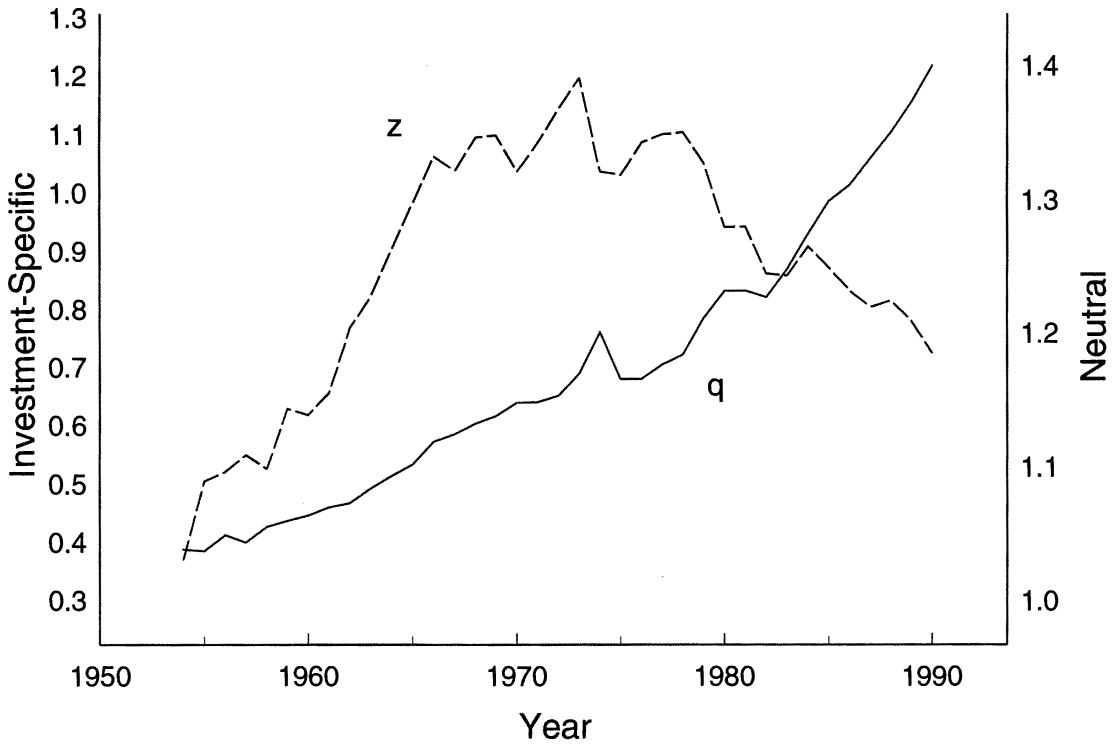
\includegraphics[width=0.8\linewidth]{fig3_technological_change.jpg}
        \vspace{-1em}
        \caption{Technological Change}
      \end{figure}
      \footnotesize
      \vspace{-1em}
      注：左轴：投资特定技术（$q$），右轴：中性技术（$z$）
    \end{column}
    \begin{column}{0.41\linewidth}

      \begin{block}{图像解读}
        \begin{itemize}
          \item $q$ 增长很快（3.21\%）
          \item $z$ 增长较慢（0.39\%）
        \end{itemize}
      \end{block}

      \begin{block}{经济现实}
        \begin{enumerate}
          \item 中性技术增长缓慢，甚至下降
                \begin{itemize}
                  \item 石油危机，导致能源价格上升
                  \item 经济滞涨，资源配置效率降低
                \end{itemize}
          \item 投资品技术进步明显
                \begin{itemize}
                  \item 计算机、通讯技术蓬勃发展
                  \item 数控机床，物流运输不断改进
                \end{itemize}
        \end{enumerate}
      \end{block}
    \end{column}
  \end{columns}
\end{frame}

\begin{frame}{Figure 4：重新理解经济增长}
  \small
  \begin{columns}[T,onlytextwidth]
    \begin{column}{0.55\linewidth}
      \begin{figure}
        \centering
        
\includegraphics[width=0.9\linewidth]{image/fig4_productivity_measures.jpg}
        \vspace{-1em}
        \caption{Productivity Measures}
      \end{figure}
      \footnotesize
      % \vspace{-1em}
      % 注：$y=z_p l = z_1 k^\alpha l^(1-\alpha) = z_2 k_e^{\alpha_e} k_s^{\alpha_s}l^{1-\alpha_e-\alpha_s}$
    \end{column}
    \begin{column}{0.41\linewidth}
      \begin{block}{图像解读}
        \begin{itemize}
          \item 水平值本质上不可比
          \item 增长率不断下降：$1.24\% \to 0.71\% \to 0.68\% \to 0.39\%$
        \end{itemize}
      \end{block}

      \begin{block}{经济现实}
        \begin{itemize}
          \item 资本积累，在一定程度上解释了增长 \\（$1.24\% \to 0.70\%$）
          \item 资本的分类，对理解增长帮助不明显 \\ （$0.71\% \to 0.68\%$）
          \item 设备资本进步，也是的影响重要因素 \\ （$0.68\% \to 0.39\%$）
        \end{itemize}
      \end{block}
    \end{column}
  \end{columns}
\end{frame}

\begin{frame}{Figure 5：设备资本存量的差异}
  \vspace{-2em}
  \begin{center}
    \begin{equation*}
      k_{e,t+1}^{M}  = (1-\delta_e) k_{e,t}^{M} + \dfrac{i_e}{p^{c}_t} \cdot \dfrac{p^{c}_t}{p^{G,e}_t} \qquad
      k_{e,t+1}^{B}  = (1-\delta_e) k_{e,t}^{B} + \dfrac{i_e}{p^{B,e}_t}
    \end{equation*}
  \end{center}
  \begin{columns}[T,onlytextwidth]
    \begin{column}{0.55\linewidth}
      \begin{figure}
        \centering
        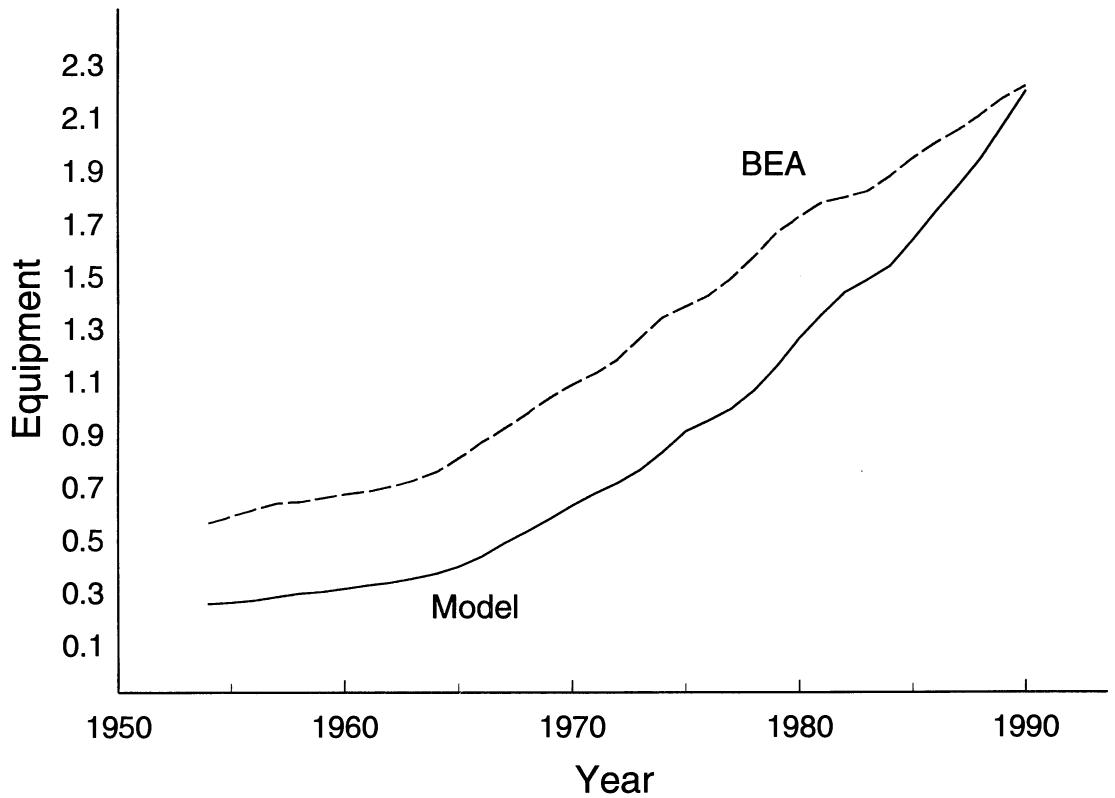
\includegraphics[width=0.8\linewidth]{fig5_equipment_stock.jpg}
        \vspace{-1em}
        \caption{Equipment Stock}
      \end{figure}
      \footnotesize
      \vspace{-1em}
      注：虚线：BEA 测算的设备资本，实线：文章测算的设备资本
    \end{column}
    \begin{column}{0.41\linewidth}

      \begin{block}{图像解读}
        \begin{itemize}
          \item BEA 测算的设备资本存量偏高
          \item Model 设备资本增速高于 BEA
        \end{itemize}
      \end{block}

      \begin{block}{经济现实}
        \begin{itemize}
          \item BEA 数据对设备价格不够充分
          \item 未被统计到的设备技术进步（$q$）
        \end{itemize}
      \end{block}
    \end{column}
  \end{columns}
\end{frame}

\begin{frame}{Figure 6：技术进步的估计误差}
  \begin{columns}[T,onlytextwidth]
    \begin{column}{0.55\linewidth}
      \begin{figure}
        \centering
        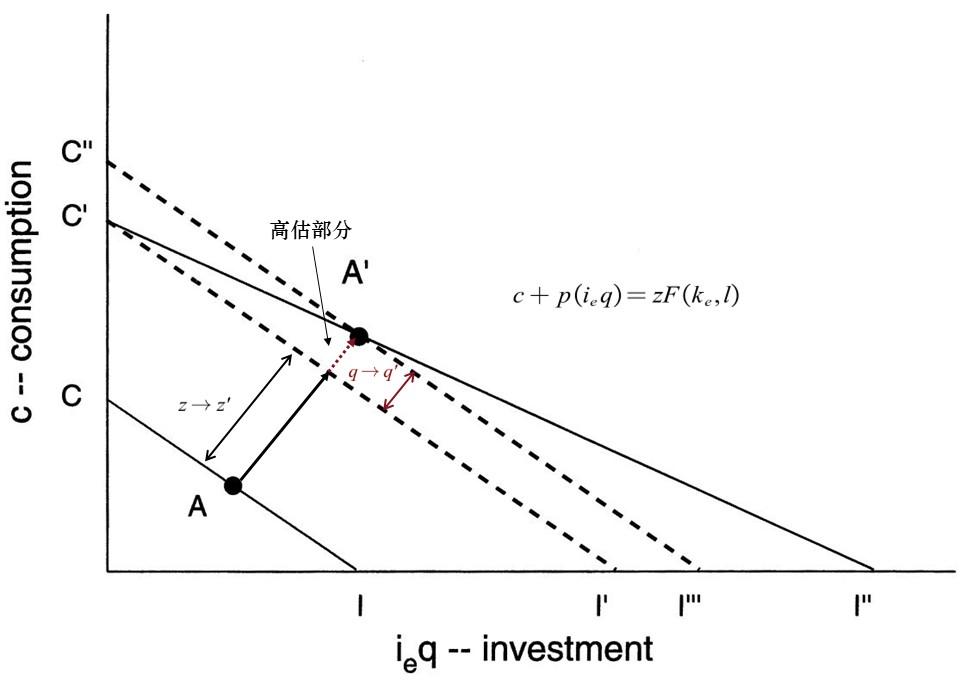
\includegraphics[width=0.9\linewidth]{image/fig6.jpg}
        \vspace{-1em}
        \caption{Measureing Netural Technological Chance.}
      \end{figure}
      \footnotesize
      \vspace{-1em}
      实线：考虑 $q$ 的消费约束（$C'-I''$）\\
      虚线：忽略 $q$ 的消费约束（$C''-I'''$）
    \end{column}
    \begin{column}{0.41\linewidth}
      \vspace{2em}
      \begin{block}{图像解读}
        \begin{itemize}
          \item 产出 $A \to A'$
          \item $C'-I''$ 中性的技术进步（$z \uparrow$）
                \begin{itemize}
                  \item 消费约束的平移
                \end{itemize}
          \item $C''-I'''$ 投资特定技术进步（$p \downarrow$）
                \begin{itemize}
                  \item 消费约束绕$C$的旋转
                \end{itemize}
        \end{itemize}
      \end{block}

      \begin{block}{经济现实}
        \begin{itemize}
          \item 忽略 $q$ 将导致 $z$ 的高估
          \item 高估部分为 $C'-I'$  与 $C''-I'''$ 的距离
        \end{itemize}
      \end{block}
    \end{column}
  \end{columns}
\end{frame}

\begin{frame}{核心结果}
  \begin{columns}[T,onlytextwidth]
    \begin{column}{0.3\linewidth}
      \datapill{实际增长}{增长约 1.24\%}
    \end{column}
    \begin{column}{0.3\linewidth}
      \datapill{$\gamma_z = 0$}{增长约 0.77\%}
    \end{column}
    \begin{column}{0.3\linewidth}
      \datapill{$\gamma_z = 0$}{增长约 0.56\%}
    \end{column}
  \end{columns}
  \vspace{1em}
  \begin{block}{结论：重新解释增长动力}
    投资特定技术进步解释增长的 60\%，中性技术增长解释剩余的 40\%
  \end{block}
\end{frame}


\section{文章启示}
% \subsection{文章价值}
\begin{frame}{为什么能发AER？}
  \small
  \setlength{\leftmarginii}{1.0em}
  \setlength{\labelsep}{0.35em}
  \begin{columns}[T,onlytextwidth]
    \begin{column}{0.45\linewidth}
      \begin{block}{重要的现实问题}
        \begin{enumerate}
          \item 长期增长从哪里来？
                \begin{itemize}
                  \scriptsize
                  \item 资本累计 + 劳动投入 + 技术进步
                  \item 三者并非相互独立，资本和劳动也可能有技术进步
                \end{itemize}
          \item 如何理解索洛悖论？
                \begin{itemize}
                  \scriptsize
                  \item 信息技术的发展，在 TFP 中难以统计
                  \item 技术的划分足够够细时，就可以观察到
                \end{itemize}
        \end{enumerate}
      \end{block}
    \end{column}

    \begin{column}{0.5\linewidth}
      \begin{block}{重要的理论创新}
        \begin{enumerate}
          \item 价格指数：技术进步的具象化
                \begin{itemize}
                  \scriptsize
                  \item 将效率提高与价格降低联系起来，技术进步可识别
                  \item 为研究技术的短期波动和投资冲击提供条件
                \end{itemize}
          \item 结构转型：单部门到多部门
                \begin{itemize}
                  \scriptsize
                  \item 将资本进行分类，并赋予价格、质量和技术等差异
                  \item 已经有多部门的雏形，是后续经济结构相关研究的基础
                \end{itemize}
        \end{enumerate}
      \end{block}
    \end{column}
  \end{columns}

\end{frame}

\begin{frame}{后续研究}
  \begin{figure}
    \centering
    
\includegraphics[width=0.8\linewidth,keepaspectratio]{\detokenize{image/文献综述.png}}
    % \caption{后续研究}
  \end{figure}

\end{frame}

\begin{frame}{我们的启发}
  \begin{enumerate}
    \item 变量的进一步细化
          \begin{itemize}
            \item 本文：将传统的 $k$，划分为 $k_e$ 和 $k_s$
            \item 其它研究：
          \end{itemize}
    \item 冲击的非对称性影响
          \begin{itemize}
            \item 本文：技术进步 $q$ 的影响对不同资本存在差异
            \item 其它研究：
          \end{itemize}
  \end{enumerate}
\end{frame}


% \begin{frame}[allowframebreaks]{参考文献}
%   \nocite{greenwood1997longrun}
%   \bibliographystyle{apalike}
%   \bibliography{references}
% \end{frame}

\end{document}
